\documentclass{standalone}
\usepackage{tikz}
\usetikzlibrary{positioning,calc}
\definecolor{uablue}{RGB}{0,61,100}
\colorlet{uablue25}{uablue!25}
\definecolor{uared}{RGB}{126,0,47}
\colorlet{uared25}{uared!25}
\definecolor{uagreen}{RGB}{0,126,1}
\colorlet{uagreen25}{uagreen!25}
\begin{document}
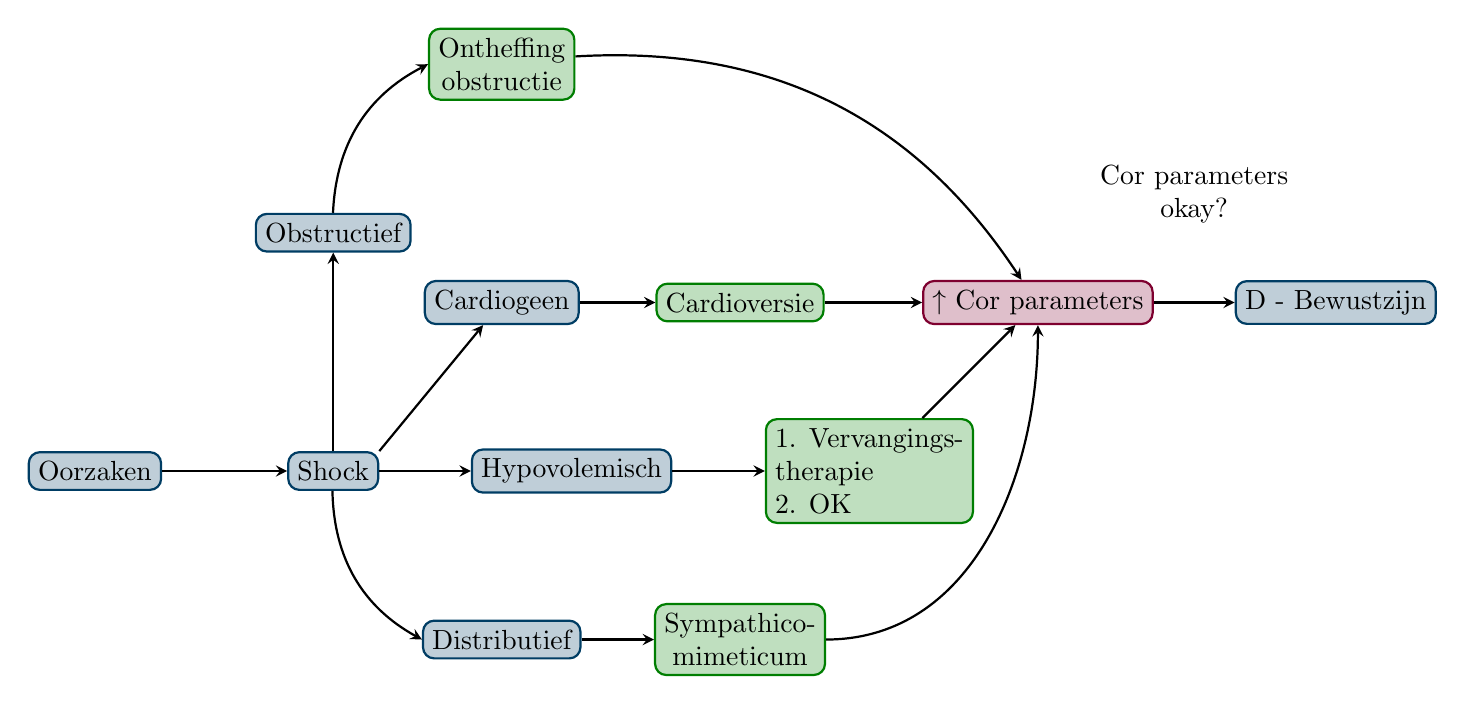
\begin{tikzpicture}[%
    blank/.style={inner sep=0,opacity=0,text opacity=1},
                    node distance=20ex,bluebox/.style={draw=#1,fill=#1!25,thick,rounded corners},
                    bluebox/.default=uablue,
                    every node/.style={bluebox}
    ]
    \node (oorzaken) {Oorzaken};
    \node[right of=oorzaken,bluebox] (shock) {Shock};
    %%% Verschillende type shocks
    \node[below right of=shock] (distr_shock) {Distributief};
    \node[right of=shock] (hypovol_shock) {Hypovolemisch};
    \node[above right of=shock] (car_shock) {Cardiogeen};
    \node[above of=shock] (obstruc_shock) {Obstructief};
    %%% Oplossingen
    \node[bluebox=uagreen,right of=distr_shock,align=center] (sympatico) {Sympathico-\\mimeticum};
    \node[bluebox=uagreen,right of=hypovol_shock,align=left,node distance=25ex] (vervang_therap) 
        {1. Vervangings-\\therapie\\
         2. OK
        };
    \node[bluebox=uagreen,right of=car_shock] (carversie) {Cardioversie};
    \node[bluebox=uagreen,above right of=obstruc_shock,align=center] (ontheffing_obstruc) {Ontheffing\\obstructie};
    %%% Vitale parameters
    \node[bluebox=uared,above right of=vervang_therap] (car_par) {$\uparrow$ Cor parameters};
    %%%
    \node[right of=car_par,node distance=25ex] (D_abcde) {D - Bewustzijn};
    \path[draw,->,>=stealth,thick] 
        (oorzaken) edge (shock)
        %%% naar subdivisies shock
        (shock) edge[bend right]  (distr_shock.west) 
        (shock.north east) edge (car_shock) 
        (shock) edge (obstruc_shock)
        (shock) edge (hypovol_shock)
        %%% behandelingen van subdivies
        (distr_shock) edge (sympatico)
        (hypovol_shock) edge (vervang_therap) 
        (car_shock) edge (carversie)
        (obstruc_shock) edge[bend left] (ontheffing_obstruc.west)
        %%% naar cor parameters
        (sympatico) edge [out=0,in=-90] (car_par)
        (vervang_therap) edge (car_par)
        (carversie) edge (car_par)
        (ontheffing_obstruc) edge[bend left] (car_par)
        (car_par) -- (D_abcde) node[align=center,midway,yshift=1cm,anchor=south,blank] (Okay) {Cor parameters\\ okay?}
        ;
\end{tikzpicture} 
\end{document}
